%%%%%%%%%%%%%%%%%%%%%%%%%%%%%%%%%%%%%%%%%
% Beamer Presentation
% LaTeX Template
% Version 1.0 (10/11/12)
%
% This template has been downloaded from:
% http://www.LaTeXTemplates.com
%
% License:
% CC BY-NC-SA 3.0 (http://creativecommons.org/licenses/by-nc-sa/3.0/)
%
%%%%%%%%%%%%%%%%%%%%%%%%%%%%%%%%%%%%%%%%%

%----------------------------------------------------------------------------------------
%	PACKAGES AND THEMES
%----------------------------------------------------------------------------------------

\documentclass{beamer}

\mode<presentation> {

% The Beamer class comes with a number of default slide themes
% which change the colors and layouts of slides. Below this is a list
% of all the themes, uncomment each in turn to see what they look like.

%\usetheme{default}
%\usetheme{AnnArbor}
%\usetheme{Antibes}
%\usetheme{Bergen}
%\usetheme{Berkeley}
%\usetheme{Berlin}
%\usetheme{Boadilla}
%\usetheme{CambridgeUS}
%\usetheme{Copenhagen}
%\usetheme{Darmstadt}
%\usetheme{Dresden}
%\usetheme{Frankfurt}
%\usetheme{Goettingen}
%\usetheme{Hannover}
%\usetheme{Ilmenau}
%\usetheme{JuanLesPins}
%\usetheme{Luebeck}
\usetheme{Madrid}
%\usetheme{Malmoe}
%\usetheme{Marburg}
%\usetheme{Montpellier}
%\usetheme{PaloAlto}
%\usetheme{Pittsburgh}
%\usetheme{Rochester}
%\usetheme{Singapore}
%\usetheme{Szeged}
%\usetheme{Warsaw}

% As well as themes, the Beamer class has a number of color themes
% for any slide theme. Uncomment each of these in turn to see how it
% changes the colors of your current slide theme.

%\usecolortheme{albatross}
%\usecolortheme{beaver}
%\usecolortheme{beetle}
%\usecolortheme{crane}
%\usecolortheme{dolphin}
%\usecolortheme{dove}
%\usecolortheme{fly}
%\usecolortheme{lily}
%\usecolortheme{orchid}
%\usecolortheme{rose}
%\usecolortheme{seagull}
%\usecolortheme{seahorse}
%\usecolortheme{whale}
%\usecolortheme{wolverine}

%\setbeamertemplate{footline} % To remove the footer line in all slides uncomment this line
%\setbeamertemplate{footline}[page number] % To replace the footer line in all slides with a simple slide count uncomment this line

%\setbeamertemplate{navigation symbols}{} % To remove the navigation symbols from the bottom of all slides uncomment this line
}

\usepackage{graphicx} % Allows including images
\usepackage{booktabs} % Allows the use of \toprule, \midrule and \bottomrule in tables

%----------------------------------------------------------------------------------------
%	TITLE PAGE
%----------------------------------------------------------------------------------------

\title[NQA Seminar]{NQA Seminar: ProPara} % The short title appears at the bottom of every slide, the full title is only on the title page

\author{Ahmed Sohail Anwari, Anan Sch{\"u}tt} % Your name
\institute[UdS] % Your institution as it will appear on the bottom of every slide, may be shorthand to save space
{
University of Saarland\\ % Your institution for the title page
\medskip
\textit{s8ahanwa, s8anscue@stud.uni-saarland.de} % Your email address
}
\date{\today} % Date, can be changed to a custom date

\begin{document}

\begin{frame}
\titlepage
\end{frame}

\begin{frame}
\frametitle{Overview}
\tableofcontents
\end{frame}

\section{ProPara Dataset}
\begin{frame}
\begin{itemize}
\item Procedural text, try to track objects during the paragraph.
\item ~2k training, ~300 testing samples.
\end{itemize}
\begin{figure}[htp]
\centering
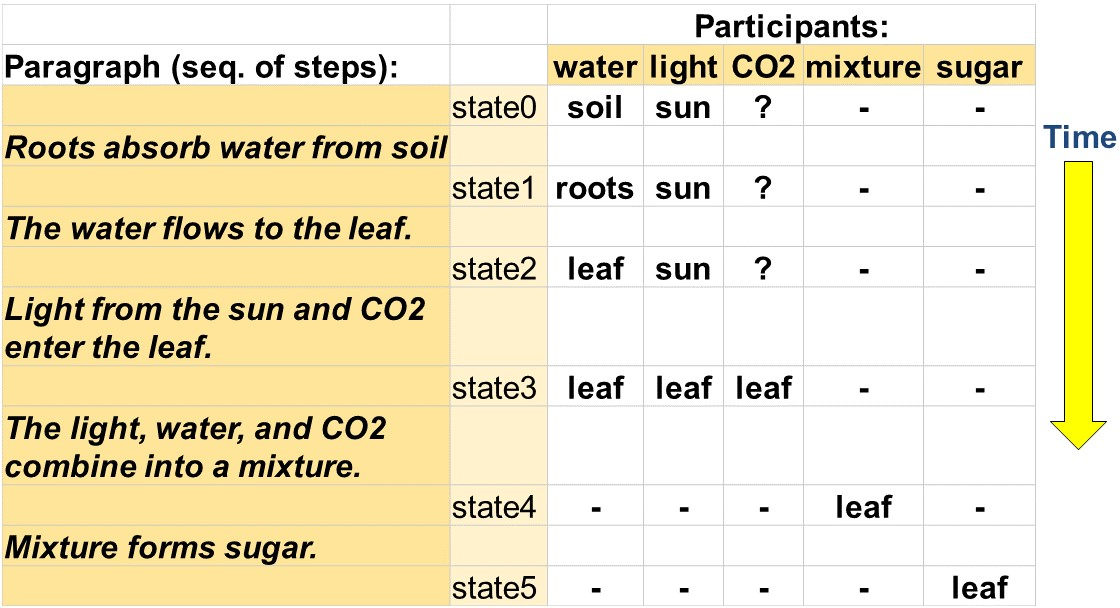
\includegraphics[width=.4\textwidth]{img/propara.jpg}
\end{figure}
\frametitle{ProPara Dataset}

\end{frame}

\section{Models}

\begin{frame}
\frametitle{ProLocal}
\begin{figure}[htp]
\centering
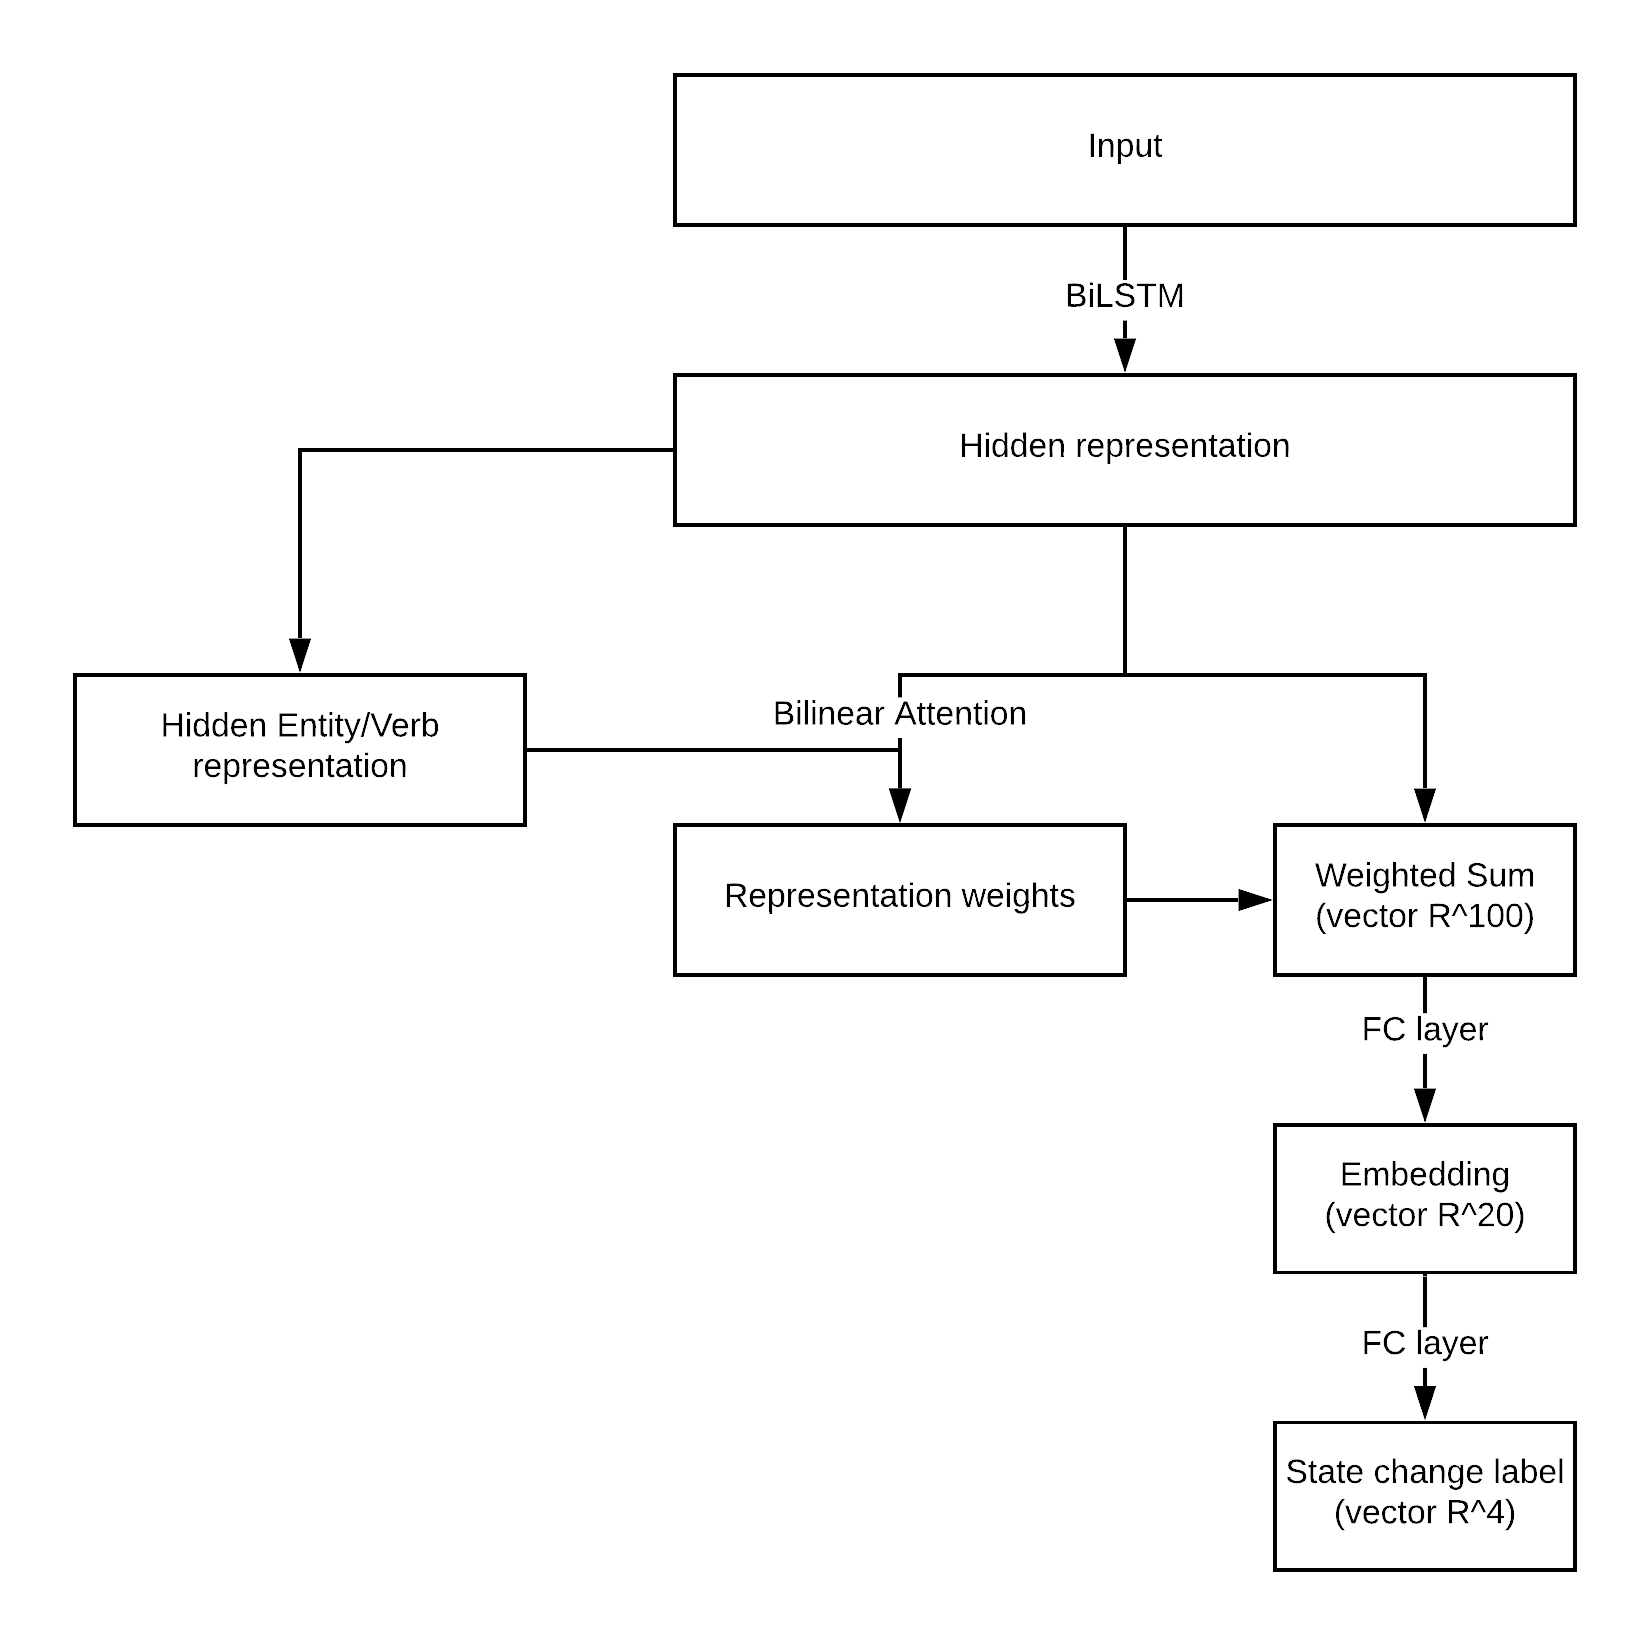
\includegraphics[width=.5\textwidth]{img/prolocal.png}
\end{figure}
\end{frame}

\begin{frame}
\frametitle{ProLocal + BERT}
\end{frame}

\section{Semi-supervised Learning}
\begin{frame}
\frametitle{Pseudo-label}
\begin{figure}[htp]
\centering
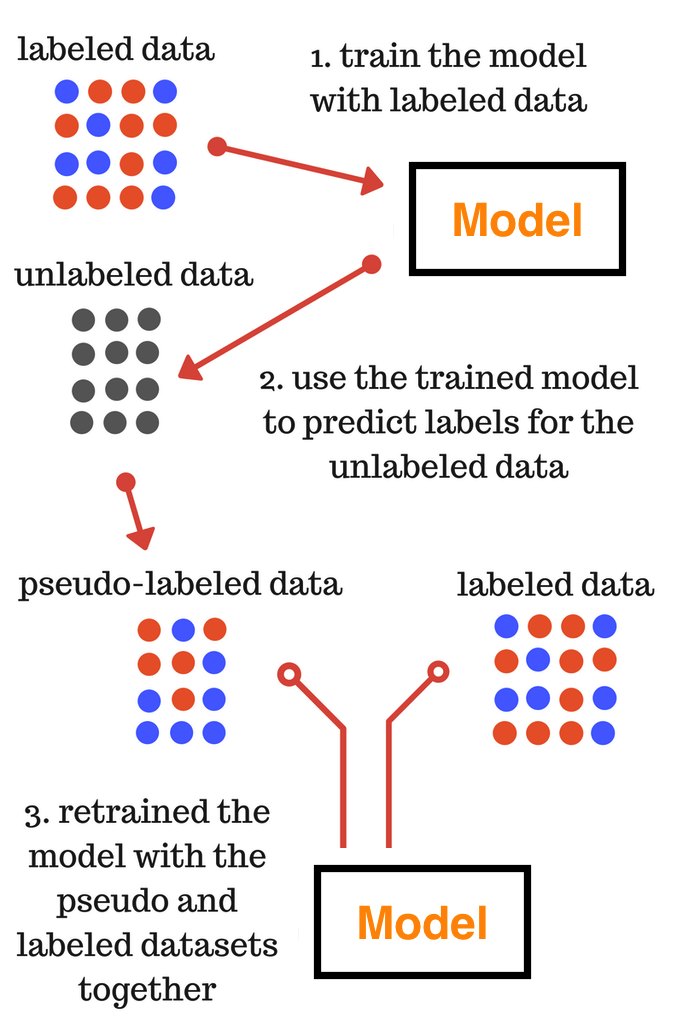
\includegraphics[width=.4\textwidth]{img/pseudo-labeling.png}
\end{figure}
\end{frame}

\begin{frame}
\frametitle{Learning by Association}
\begin{figure}[htp]
\centering
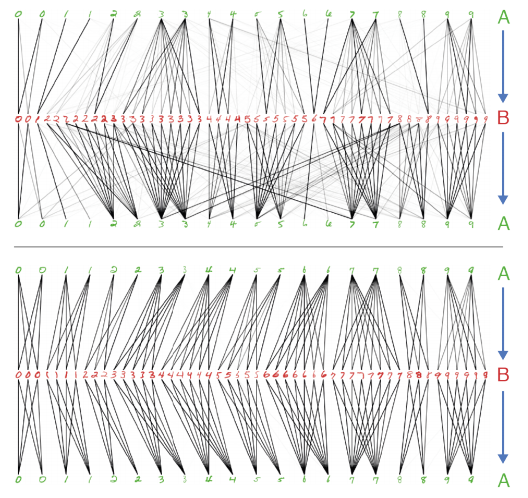
\includegraphics[width=.65\textwidth]{img/association.png}
\end{figure}
\end{frame}

\begin{frame}
\frametitle{Learning by Association}
\begin{itemize}
\item Given labeled samples $A$, unlabeled samples $B$
\item Calculate embeddings using NN, $E_A$, $E_B$
\item Similarity between samples given by $E_{A_i} \cdot E_{B_j} =: M_{ij}$
\item Define walker randomly walking between labeled and unlabeled samples by this similarity
\item Probability of walking from $A_i$ to $B_j = P^{AB}_{ij} = \frac{exp(M_{ij})}{\sum_k exp(M_{ik})}$, and similarly $P^{BA}$
\item Probability of round-trip walking is $P^{ABA} := P^{AB}P^{BA}$
\item Probability of ``correct'' walks is $\frac{1}{|A|}\sum_{i \sim j}P^{ABA}_{ij}$ 
\end{itemize}
\end{frame}

\section{Results}
\begin{frame}
\frametitle{Results - Learning by Association}
F1 scores on test set
\begin{center}
\begin{tabular}{|c|c|c|}
	\hline
	 & without unlabeled & with unlabeled\\
	\hline
	256 labeled & 0.353 (0.035) & 0.400 (0.044) \\
	512 labeled & 0.423 (0.042) & 0.436 (0.024) \\
	all labeled & 0.522 (0.018) & 0.535 (0.015) \\
	\hline
\end{tabular}
\end{center}
\end{frame}

\section{Outlook}
\begin{frame}
\frametitle{Outlook}
\begin{itemize}
\item Apply SSL on ProLocal + BERT model
\item Use other similar datasets as unlabeled samples
\end{itemize}
\end{frame}

\end{document}